\chapter{Snelast}
Ved beregning af belastninger på en given konstruktion, så skal man også tage stilling til snelasten. Snelasten på tilbygningen regnes med formlen for vedvarende/midlertidig dimensioneringstilfælde:

$s = \mu_i \cdot C_e  \cdot  C_t \cdot s_k$

hvor

\begin{itemize}
\item $\mu_i$ = formfaktor.
\item $C_e$ = eksponeringsfaktor.
\item $C_t$ = termisk faktor
\item $s_k = karakteristisk snelast på jorden$
\end{itemize}


\section{Formfaktor}
Formfaktoren afhænger af tagtype og dens hældning. Tilbygningen er beklædt med et saddeltag med følgende vinkler som kan ses på figur 1: 

\begin{figure}[H] 
\centering
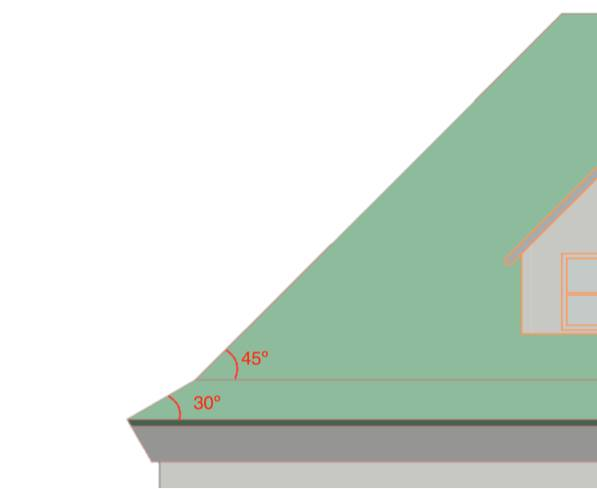
\includegraphics[width=0.60\textwidth]{billeder/SnelastFigur1}
\caption{Sadeltag med to forskellige skråninger og dermed to hældninger.}
\label{fig:SF1}
\end{figure}

Formfaktoren inddeles i tre dele; den ene med hældning på 30º, den anden med en hældning på 45º og til sidst det flade tagstykke. Form faktoren for den skrå hældning med 30º er 0,8. For den skrå hældning med 45º er værdien 0,4 og for det flade tag er værdien 0,8. 

\section{Eksponeringsfaktor}
Denne faktor er afhængig af omgivelserne omkring tilbygningen, men også dimensionerne på bygningen spiller en rolle. Deraf kommer formlen:

$C_e = C_{top} \cdot  C_s$

Topografien inddeles i enten vindblæst, normal eller afskærmet, alt efter hvor blottet konstruktionen. Da tilbygningen delvis er afskærmet og delvis vindblæst, så vælges der her den maksimale mulige værdi for topografien for at tage stilling til den værst mulige belastning der måtte forekomme. Værdien for topografien sættes dermed til 1,25.

Faktoren for dimensionen af konstruktionen sættes til at være lig med 1,0. Dette skyldes at den opfylder følgende sætning: $2h > l_1$, hvor $h$ svarer til højden af konstruktionen og $l_1$ svarer til den længste side af bygningen.

Eksponeringsfaktor kommer da til at få værdien på 1,25.

\section{Termisk faktor}
Følgende faktor bruges som en reduktionsfaktor i det tilfælde hvor der er høj varmeoverførsel såsom et drivhus med glastag. Under normale omstændigheder sættes den termisk faktor til at være 1,0.

\section{Karakteristisk terrænværdi}
Denne værdi sættes til at være lig med $\SI{1}{ kN/m^2}$ i Danmark

\section{Beregning af snelast}
De fundende faktor og variabler kan nu bruges til at finde snelasten på tilbygningen. Værdierne kan findes i tabellen forneden:

\begin{table}[H]
\centering
\begin{tabular}{|l|c|c|}
\hline
\textbf{Beskrivelse}       & \textbf{Symbol} & \textbf{Værdi}                                                                                    \\ \hline
Formfaktor                 & $\mu_i$               & \begin{tabular}[c]{@{}c@{}}0,8 (hældning 30º)\\ 0,4 (hældning 45º)\\ 0,8 (fladt tag)\end{tabular} \\ \hline
Eksponeringsfaktor         & $C_e$               & 1,25                                                                                              \\ \hline
- Topografi                & $C_{top}$               & 1,25                                                                                              \\ \hline
- Faktor for dimension     & $C_s$               & 1,0                                                                                               \\ \hline
Termisk faktor             & $C_t$               & 1,0                                                                                                 \\ \hline
Karakteristisk terrænværdi & $s_k$               & $\SI{1,0}{kN/m^2}$                                                                                              \\ \hline
\end{tabular}
\caption{Oversigt over de fundende værdier til beregning af snelast}
\label{tab:SLT1}
\end{table}


De forskellige værdier bruges til at beregne snelasten og følgende resultater kan ses i tabel \ref{tab:SLT2} Linjelasten er også beregnet over det stykke som sneen påvirket med.

\begin{table}[H]
\centering
\begin{tabular}{|l|c|c|c|}
\hline
\textbf{Tagdel}            & \textbf{Last} & \textbf{Længde} & \textbf{Linjelast} \\ \hline
Skrå del (hældning på 30º) & $\SI{1,0}{kN/m^2}$                      & 0,86 m $\cdot$ 2              & $\SI{1,73}{kN/m^2}$                                                                                                               \\ \hline
Skrå del (hældning på 45º) & $\SI{0,5}{kN/m^2}$                                     & 2,28 m $\cdot$ 2               & $\SI{4,55}{kN/m^2}$                                                                                                              \\ \hline
Fladt tag                  & $\SI{1,0}{kN/m^2}$                     &  5 m               & $\SI{5,0}{kN/m^2}$                                                                                                               \\ \hline
\end{tabular}
\caption{Oversigt over de forskellige laster for de forskellige dele som taget er blevet inddelt i.}
\label{tab:SLT2}
\end{table}


\section{Snelast fra sneophobning}
For bygningskonstruktioner som både udsættes for sne og vind, så regnes der med en ekstra lastarrangement. Vindsiden på sadeltaget vil have en formfaktor på nul, mens læsiden vil have en formfaktor afhængig af hældningen. Men inden der tages hensyn til den ekstra lastarrangement, så skal følgende sætninger være opfyldte:





\begin{enumerate}
\item bygningens orientering vender mod den østlige retning (fra NNØ til SØ)
\item facadehøjden i vindsiden er højst 10 m.
\item bygningens længde på tværs af vindsiden er to gange større end bygningens kiphøje
\item bygningens dybde er større end bygningens kiphøjde
\item terrænnet i vindsiden er åben i en afstand på 400 m.
\end{enumerate}

Da tilbygningen til Strøybergs Palæ opfylder alle betingelserne, så skal der regnes med ekstra last.  Igen ses der på figur 1, da de forskellige formfaktor som bruges til at udregne snelasten afhænger af hældningen på taget. For et tag med hældningen fra 15º til 30º beregnes formfaktoren til at være lig med 1,2. Derimod beregnes formfaktoren til at være 0,60 for taget med hældningen 45º. 

Til beregning af den ekstra snelast bruges den samme formel som tidligere anvendt i starten af kapitlet. Igen bruges denne formel til at beregne den ekstra snelast, formfaktoren er blot ændret:

$s = \mu_i \cdot C_e  \cdot  C_t \cdot s_k$

Resultatet kan ses i tabel \ref{tab:SLT3} hvor linjelasten også er skrevet ind.

\begin{table}[H]
\centering
\begin{tabular}{|l|c|c|c|}
\hline
\textbf{Tagdel}            & \textbf{Last} & \textbf{Længde} & \textbf{Linjelast} \\ \hline
Skrå del (hældning på 30º) & $\SI{0,75}{kN/m^2}$                      & 0,86 m $\cdot$ 2              & $\SI{2,59}{kN/m^2}$                                                                                                               \\ \hline
Skrå del (hældning på 45º) & $\SI{0,5}{kN/m^2}$                                     & 2,28 m $\cdot$ 2               & $\SI{6,82}{kN/m^2}$                                                                                                              \\ \hline
\end{tabular}
\caption{Oversigt over de ekstra snelaster der fremkommer ved låsiden ved vindblæst.}
\label{tab:SLT3}
\end{table}

